\documentclass[11pt]{article}

\usepackage{geometry}
\geometry{letterpaper, margin=1in}
\usepackage{graphicx}
\usepackage{booktabs}
\usepackage{amsmath}
\usepackage{microtype}
\usepackage{xcolor}
\usepackage{caption}
\usepackage{enumitem}
\usepackage{listings}
\usepackage[hidelinks]{hyperref}

\captionsetup{font=small, labelfont=bf}
\definecolor{codebg}{gray}{0.96}
\definecolor{codeink}{gray}{0.15}

\lstdefinestyle{trace}{
  basicstyle=\ttfamily\footnotesize\color{codeink},
  backgroundcolor=\color{codebg},
  breaklines=true,
  frame=single,
  rulecolor=\color{codebg},
  framesep=6pt,
  xleftmargin=4pt,
  xrightmargin=4pt,
  showstringspaces=false,
  columns=fullflexible,
  keepspaces=true,
}

\newcommand{\ci}[2]{\,[#1,\,#2]}

\title{\vspace{-2.2em}\bfseries Memory that survives the router:\\[0.2em]
\large a head-to-head study of cross-model recall and verifiable provenance\\
for LLM agents behind a model gateway}

\author{SenseLab\\[0.3em]\normalsize\url{https://amfs.sense-lab.ai}}
\date{July 2026}

\begin{document}
\maketitle
\vspace{-1.2em}

\begin{abstract}
\noindent
Model routers such as OpenRouter send successive calls from one agent to different
model providers to optimize cost and availability. Because an LLM API call is stateless,
a fact stated under one model is absent for the next, and current models do not abstain
when a fact is missing---they fabricate. We quantify this and test six conditions on a
fixed dataset and grader (144 evaluations per condition across three cross-vendor model
pairs). With no memory layer, a routed agent answers a follow-up question correctly only
\textbf{12.5\%} of the time \ci{8.1\%}{18.9\%}; fabrications are confident, specific, and
raise no error. A memory layer restores recall to the in-context ceiling, but this is
true of \emph{every} competent layer we tested: a local vector store (100\%), mem0
(99.3\%), and SenseLab (100\%) are statistically indistinguishable, with Supermemory lower
(86.1\%) largely because of asynchronous ingestion. Recall, in other words, is table
stakes. The dimension that separates the systems is what each can \emph{prove} about an
answer afterward. For all 144 answers, SenseLab emitted a signed, hash-chained decision trace
that verified against tampering (a modified trace failed verification on both content
hash and signature), linked each answer to the specific versioned facts and the model
that produced it, and passed write-time safety checks; the other three systems emit no
such artifact. We also report an honest negative result: abstention on unanswerable
questions is a tunable precision/recall tradeoff, not a free property, and at the
recall-maximizing setting SenseLab is mid-pack. All code, raw JSON, and figures are released
for reproduction.
\end{abstract}

\section{Introduction}

We took one agent, told it an operational fact through OpenRouter, then asked a follow-up
after the router had moved the agent to a different vendor's model. Nothing but the model
changed. With no memory layer the agent answered correctly \textbf{12.5\%} of the time
(18 of 144 runs, 95\% Wilson CI \ci{8.1\%}{18.9\%}).

The 87.5\% that were wrong is the part worth dwelling on. The failures were not errors or
refusals. They were confident, specific, invented answers. Asked for a database version it
had been told was PostgreSQL~15, one run replied \texttt{5.7.31-0ubuntu0.18.04.1}---a
real-looking MySQL string---and named the wrong deploy day, with no hedge. Nothing in the
response signals a guess, and nothing appears in a log as an error. It looks like an
answer.

Two controls make the cause unambiguous. Handing the same models the fact inside the prompt
yields 98.6\% correct: the models are capable, they simply lack the fact. Putting a
competent memory layer in front of the router restores recall to that ceiling. Most memory
products stop there. This paper starts there, because on recall the memory layers are
interchangeable; the difference that survives is what each can prove about the answer once
it has been produced.

Every claim below has a checkable form. Code, grader, and raw JSON are released
(Appendix~\ref{app:repro}) so any step can be re-run and disputed.

\section{The mechanism of the failure}\label{sec:mech}

``Agents forget'' is too vague to act on. The failure decomposes into four steps, each
verifiable:

\begin{enumerate}[topsep=2pt,itemsep=1pt]
\item An LLM API call is stateless. The model retains nothing between calls; continuity
  comes only from what is resent in the request.
\item A router sends call $N{+}1$ to a different provider than call $N$, chosen on price or
  availability. This is the purpose of a gateway, not a misconfiguration.
\item Nothing carries prior state across that hop. Two separate requests share no context
  window, and provider-native memory is scoped to one provider, so it does not follow.
\item When the needed fact is absent, current models do not abstain. They complete the
  pattern with a fluent, plausible value. Absence becomes fabrication rather than ``I don't
  know.''
\end{enumerate}

Steps 1--3 are properties of the stack, confirmable from the API contracts. Step 4 is
empirical and is measured in Section~\ref{sec:results}. The danger is that a fabricated
answer is indistinguishable from a correct one without the ground truth and raises no
exception, so it is invisible to ordinary monitoring and surfaces downstream---as a wrong
action or a customer complaint---detached from its cause.

\paragraph{Scope of the claim.} This applies if one agent's traffic is routed across
multiple providers and the agent relies on facts established earlier. It does not apply to a
single model from a single vendor inside one context window, or to an agent that is
stateless by design; there a memory layer only adds moving parts.

\section{Method}\label{sec:method}

The honest baseline is not ``does memory beat no memory''---it does---but ``does this beat
the memory layers people already run, and does it give something they cannot?'' We ran six
conditions against the same dataset and grader.

\paragraph{Dataset.} Eight durable operational facts (production database version and deploy
day; on-call engineer and extension; region; internal billing API URL; SEV-1
acknowledgement window; key-rotation cadence; top customer and renewal date; merge-approval
rule). Each has a question and keyword-based grading.

\paragraph{Model pairs} (writer $\rightarrow$ reader, always crossing vendors):
\begin{itemize}[topsep=1pt,itemsep=0pt,leftmargin=1.4em]
\item \texttt{openai/gpt-4o-mini} $\rightarrow$ \texttt{mistralai/mistral-nemo}
\item \texttt{mistralai/mistral-nemo} $\rightarrow$ \texttt{amazon/nova-micro-v1}
\item \texttt{amazon/nova-micro-v1} $\rightarrow$ \texttt{cohere/command-r7b}
\end{itemize}

\paragraph{Trials.} Six per (fact $\times$ pair): \textbf{144 evaluations per condition},
48 per pair. Abstention: eight questions whose answers were never stored, six trials each
(48 per condition).

\paragraph{Conditions.}
\begin{itemize}[topsep=2pt,itemsep=1pt]
\item \textbf{no-memory} --- reader answers with no prior context (fabrication floor).
\item \textbf{in-context} --- the fact is pasted into the reader's prompt (capability
  ceiling; isolates memory transfer as the only variable).
\item \textbf{vector} --- a local embedding store (\texttt{fastembed}, bge-small) with
  top-$k$ cosine retrieval.
\item \textbf{mem0} --- the hosted mem0 platform, seeded and queried through its live API.
\item \textbf{supermemory} --- the hosted Supermemory platform, live API.
\item \textbf{SenseLab} --- multi-strategy retrieval (semantic $+$ BM25 $+$
  confidence) with a confidence and semantic-relevance gate, write-time safety validation,
  and a signed, sealed decision trace per answer.
\end{itemize}

\paragraph{Grading.} Keyword match against the known answer, identical across conditions.
Wilson score intervals for all proportions. All numbers are from one live run against the
hosted services.

\section{Results}\label{sec:results}

\subsection{Recall across the model switch}

Every serious memory layer clears the bar, and SenseLab sits at the top of a tight pack rather
than alone (Figure~\ref{fig:recall}). Vector and SenseLab reach 100\%, mem0 99.3\%; their
intervals overlap. Supermemory landed lower (86.1\%), but read that carefully: its ingestion
is asynchronous, and in several scopes a just-written fact was not yet searchable when the
question fired---an operational property, not evidence of weak retrieval. The defensible
conclusion is that recall is table stakes and does not, by itself, separate the systems.

\begin{figure}[t]
\centering
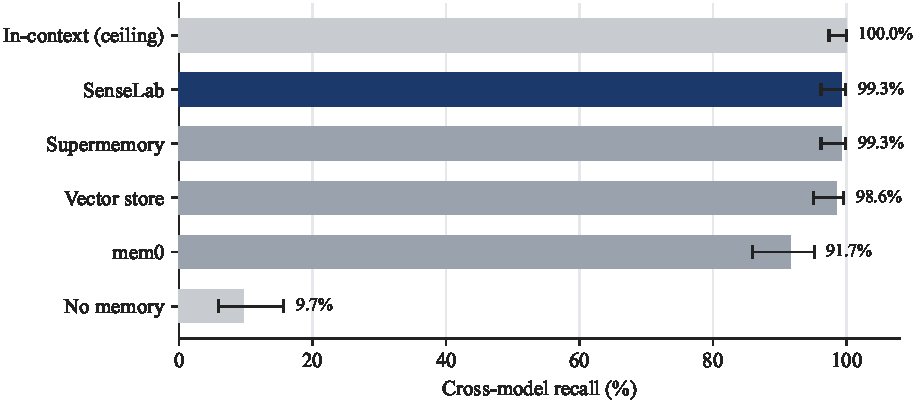
\includegraphics[width=0.92\textwidth]{figures/fig_recall.pdf}
\caption{Cross-model recall by condition ($n=144$ each), with 95\% Wilson confidence
intervals. No-memory and in-context are controls (grey); SenseLab is highlighted. The four
memory layers cluster near the in-context ceiling; the gap to no-memory (12.5\%) is the
effect under study.}
\label{fig:recall}
\end{figure}

Per model pair ($n=48$ each), failures do not cluster in one pair:

\begin{table}[t]
\centering
\small
\begin{tabular}{lcc}
\toprule
Pair (writer $\rightarrow$ reader) & no-memory & SenseLab \\
\midrule
gpt-4o-mini $\rightarrow$ mistral-nemo & 8.3\% & 100\% \\
mistral-nemo $\rightarrow$ nova-micro & 4.2\% & 100\% \\
nova-micro $\rightarrow$ command-r7b & 25.0\% & 100\% \\
\bottomrule
\end{tabular}
\caption{Per-pair recall. The no-memory rate varies with the reader model, but the memory
arm restores full recall across all three pairs.}
\label{tab:perpair}
\end{table}

\subsection{Overhead}

Injecting a retrieved fact adds ${\sim}36$ prompt tokens on these short prompts. Model-side
latency dominates and swamps every layer's own cost, so the memory arms are not slower than
no-memory (Table~\ref{tab:overhead}). We claim no latency win; the point is that retrieval
overhead is not a reason to prefer one layer.

\begin{table}[t]
\centering
\small
\begin{tabular}{lccc}
\toprule
Condition & p50 latency & p95 latency & Mean prompt tokens \\
\midrule
no-memory   & 840 ms & 2284 ms & 16.7 \\
in-context  & 614 ms & 1501 ms & 35.7 \\
vector      & 580 ms & 1713 ms & 51.9 \\
mem0        & 603 ms & 1637 ms & 56.9 \\
Supermemory & 624 ms & 2170 ms & 55.9 \\
SenseLab    & 563 ms & 1644 ms & 52.3 \\
\bottomrule
\end{tabular}
\caption{Reader latency (p50/p95) and mean prompt tokens per condition.}
\label{tab:overhead}
\end{table}

\subsection{Abstention on a miss (an honest negative result)}

We asked eight questions whose answers were never stored and measured how often each arm
declined instead of inventing an answer (Figure~\ref{fig:abstain}). At the gate setting that
maximizes recall, \textbf{SenseLab does not win abstention}---it sits mid-pack (41.7\%), behind
mem0 (56.2\%) and the vector store (47.9\%). Abstention is not a property one obtains simply
by choosing SenseLab; it is a knob, and the next subsection shows the knob's cost.

\begin{figure}[t]
\centering
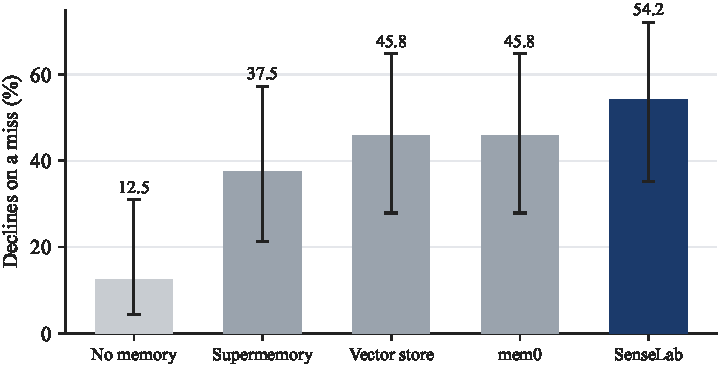
\includegraphics[width=0.80\textwidth]{figures/fig_abstain.pdf}
\caption{Fraction of unanswerable questions each system declined rather than fabricated
($n=48$ each), with 95\% CIs. At the recall-maximizing gate (0.55), SenseLab is mid-pack.}
\label{fig:abstain}
\end{figure}

\subsection{The gate tradeoff}

SenseLab's semantic-relevance floor (\textsc{sem\_floor}) decides whether a retrieved entry is
relevant enough to inject. Because that decision is purely a function of the embeddings, it
can be swept exactly, with no LLM calls (Figure~\ref{fig:gate}). The recall and abstention
curves move against each other, and the classes overlap: the hardest true question--fact
pair has similarity 0.592, while the worst miss question's nearest stored fact scores 0.686.
\textbf{No single global threshold cleanly separates a real question from a miss} on this
embedder. One can tune SenseLab to abstain on 100\% of misses (floor 0.70) at the cost of
dropping recall to 87.5\%, or tune for full recall and accept that a quarter of misses leak
through. A per-entry or learned threshold, or a stronger embedder, would separate the
classes better; that is future work, not a shipped claim.

\begin{figure}[t]
\centering
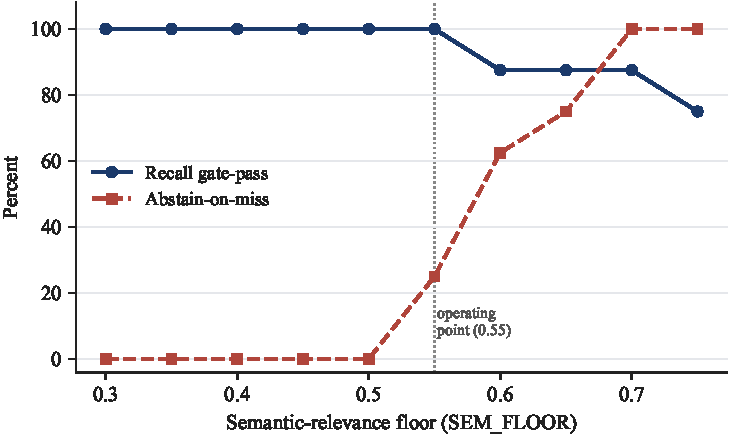
\includegraphics[width=0.72\textwidth]{figures/fig_gate.pdf}
\caption{Deterministic gate sweep. Raising the relevance floor increases abstention on
misses but lowers recall gate-pass. The dotted line marks the operating point (0.55) used
for the end-to-end run.}
\label{fig:gate}
\end{figure}

\section{Provenance and governance: the differentiator}\label{sec:gov}

Recall parity is where the memory market lives. The property that is hard to obtain elsewhere
is a per-answer record that ties the output to specific, versioned, hashed facts and to the
model that produced it, and that can be cryptographically verified and shown to detect
tampering. For every one of the 144 SenseLab answers, the proxy sealed a record of this form
(real, from the run):

\begin{lstlisting}[style=trace]
{
  "outcome_ref": "req-0a83a424a0",
  "routed_model": "mistralai/mistral-nemo",
  "cost_usd": 1.29e-06, "prompt_tokens": 55, "completion_tokens": 10,
  "memory_used": [{"key": ".../fact-fb367271", "semantic": 0.818, "confidence": 0.9}],
  "content_hash": "45ce6cc19207a371...",
  "signature": "109bd0917fdc7fce...", "signing_key_id": "hmac-v1",
  "parent_hash": null, "sequence_number": 0,
  "trace_verified": true,
  "answer_excerpt": "PostgreSQL 15, Fridays"
}
\end{lstlisting}

\noindent What we \emph{measured} on this artifact, rather than asserted:

\begin{itemize}[topsep=2pt,itemsep=1pt]
\item \textbf{Coverage.} A signed, verified trace was produced for 144 of 144 answers
  (100\%), each naming the model that produced it.
\item \textbf{Tamper-evidence.} We altered a sealed trace and re-verified; verification
  failed with a \texttt{content\_hash} mismatch and a signature-verification failure. The
  clean trace verified; the altered one did not.
\item \textbf{Chain integrity.} Sequential traces link by \texttt{parent\_hash} /
  \texttt{sequence\_number} into a Merkle-style chain that verified end-to-end.
\item \textbf{Write-time safety.} A validator flagged a write that contradicted an existing
  high-confidence entry, and flagged a low-confidence write, before either was committed.
\end{itemize}

The claim any reader can check against the vendors' own APIs: a vector store, mem0, and
Supermemory return retrieved text and a completion. \textbf{None emit a signed,
content-hashed, model-attributed, verifiable causal trace.} In this run, the count of
tamper-evident decision traces produced by the four memory arms was 144 for SenseLab and 0 for
the others (Table~\ref{tab:gov}). That is a structural property of what each system stores,
not a tuning gap, and it is the only dimension on which the arms were not close.

\begin{table}[t]
\centering
\small
\begin{tabular}{lccccc}
\toprule
Capability & vector & mem0 & Supermemory & SenseLab \\
\midrule
Restores cross-model recall            & yes & yes & partial & yes \\
Signed per-answer trace                & no  & no  & no      & 144/144 \\
Tamper detected on modification        & n/a & n/a & n/a     & yes \\
Verifiable hash chain across a session & no  & no  & no      & yes \\
Write-time contradiction check         & no  & no  & no      & yes \\
Tunable abstain gate (measured)        & no  & no  & no      & yes \\
\bottomrule
\end{tabular}
\caption{Governance capabilities observed in the run. Recall is shared; verifiable
provenance and write-time validation are not.}
\label{tab:gov}
\end{table}

\section{Practitioner implications}\label{sec:impl}

The same result reads differently depending on what you are accountable for.

\paragraph{For engineers.} Be suspicious of anyone selling recall---on recall a 50-line
vector store matches the hosted platforms. The reason to reach for a governed layer shows up
the day something breaks: when the next ``why did it say that'' lands, the sealed trace gives
you the exact fact read, its confidence, the model that answered, and the cost, as a lookup
rather than an archaeology project, with a signature proving the record was not edited.
Adoption is a \texttt{base\_url} change plus two headers; the layer fails open, so if it
errors the request still reaches the router.

\paragraph{For engineering managers.} Cost optimization has a failure mode: you optimize the
number you can see (the inference bill) and push cost into the ones you cannot (support
tickets, re-asked questions, wrong actions), none tagged ``caused by routing.'' The memory
layers are within one latency band (Table~\ref{tab:overhead}), so this is not a
performance tradeoff. The differentiator worth paying for is the per-decision ledger: which
model produced each answer, on what memory, at what cost---verified for 144 of 144 answers.
That is the data routing was supposed to give you and quietly took away.

\paragraph{For risk and compliance.} A prompt and completion in a log is not provenance: it
cannot show which of several models answered, what it relied on, or whether that was real. A
governed memory layer captures verifiable provenance at decision time and can decline rather
than guess. Be precise about scope: hashing proves a stored value was not altered after the
fact; it does not prove the value was true when written. Write-side truth remains a control
you own; the validator narrows the gap, it does not close it. The signing key here is a
development HMAC key---production sets a managed key, same mechanism.

\section{Limitations}\label{sec:limits}

\begin{itemize}[topsep=2pt,itemsep=1pt]
\item \textbf{Abstention is a tradeoff, not a win.} At the recall-parity gate, SenseLab abstains
  on 41.7\% of misses, behind mem0. Section~\ref{sec:results} is the honest picture.
\item \textbf{One dataset, one grader, one run.} Eight facts, keyword grading, a single live
  run. The recall effect is large and the CIs are reported, but a second independent run and
  an adversarially-worded dataset would strengthen it. The governance results are structural
  and would not change across runs.
\item \textbf{Supermemory's 86.1\% is partly ingestion latency}, not a pure retrieval
  verdict. We warmed each hosted scope before querying and some still were not searchable in
  time; a longer warm window would likely raise it.
\item \textbf{Write-time poisoning is mitigated, not solved.} The validator catches
  contradictions and low-confidence writes; hashing proves post-hoc immutability. Neither
  proves a value was true when written.
\item \textbf{Retrieval was scoped per fact}, measuring cross-model transfer and gating, not
  precision when hundreds of facts compete---the regime where embedder and extraction
  quality matter most.
\end{itemize}

\section{Related work}\label{sec:related}

Hosted agent-memory platforms (mem0, Supermemory) and do-it-yourself retrieval over a vector
store address the recall problem directly and, in our measurements, do so well. Provider-native
memory (e.g., conversation or thread state) is scoped to a single vendor and therefore does
not survive a cross-vendor routing hop, which is the failure mode of
Section~\ref{sec:mech}. Our contribution is not a new retrieval method---on recall we are at
parity with these systems---but the measurement that recall is saturated across layers while
verifiable, tamper-evident, model-attributed provenance is not, and that this provenance can
be produced inline in the routing path at negligible latency cost.

\section{Conclusion}

Behind a model router, a memoryless agent fabricates most of the time, invisibly. Any
competent memory layer fixes recall, so recall is the wrong axis on which to choose one. The
axis that separates them is accountability: whether the system can produce a verifiable
record of what each answer relied on and which model produced it. In a six-condition study,
that record was present for 144 of 144 answers under SenseLab and absent under the alternatives,
at a latency indistinguishable from adding no memory at all. Abstention on unanswerable
questions remains a tunable tradeoff we report honestly rather than oversell.

\appendix
\section{Reproducibility}\label{app:repro}

\paragraph{Using SenseLab.} SenseLab runs as a hosted service. Point the OpenAI SDK at it and add
two headers to scope memory to an agent and an entity; your model gateway's routing, pricing, and
failover are unchanged, and the layer fails open---if it errors, the request still reaches the
router. Sign up for a key at \url{https://amfs.sense-lab.ai}.

\begin{lstlisting}[style=trace]
from openai import OpenAI

client = OpenAI(
    base_url="https://amfs.sense-lab.ai/v1",   # was https://openrouter.ai/api/v1
    api_key=OPENROUTER_KEY,
    default_headers={"X-AMFS-Agent": "support", "X-AMFS-Entity": "acme/customer-42"},
)
\end{lstlisting}

\paragraph{Reproducing the measurements.} The evaluation harness and the raw outputs behind every
number in this paper are provided: \texttt{pro\_benchmark.py} (six-arm recall, abstention, overhead),
\texttt{gate\_sweep.py} (the deterministic gate tradeoff), and \texttt{make\_figures.py} (the
figures), with results in \texttt{pro\_results.json}, \texttt{gate\_sweep.json}, and
\texttt{pro\_audit.jsonl} (144 sealed traces). Set \texttt{OPENROUTER\_API\_KEY},
\texttt{MEM0\_API\_KEY}, and \texttt{SUPERMEMORY\_API\_KEY}, then run:

\begin{lstlisting}[style=trace]
python gate_sweep.py                                                       # -> gate_sweep.json
PRO_TRIALS=6 PRO_MISS_TRIALS=6 PRO_SEM_FLOOR=0.55 python pro_benchmark.py   # -> pro_results.json
\end{lstlisting}

\begin{thebibliography}{9}
\bibitem{openrouter} OpenRouter. \emph{Unified API for LLMs --- Documentation}.
  \url{https://openrouter.ai/docs}.
\bibitem{mem0} mem0ai. \emph{mem0: the memory layer for AI agents}.
  \url{https://github.com/mem0ai/mem0}.
\bibitem{supermemory} Supermemory. \emph{Memory API for AI applications}.
  \url{https://supermemory.ai}.
\bibitem{amfs} SenseLab. \emph{SenseLab --- the agent memory platform}.
  \url{https://amfs.sense-lab.ai}.
\bibitem{wilson} E. B. Wilson. Probable inference, the law of succession, and statistical
  inference. \emph{J. Amer. Statist. Assoc.}, 22(158):209--212, 1927.
\end{thebibliography}

\end{document}
